\chapter{Results}\label{ch:jscheme_results}

In this chapter,
we discuss the application of the IMSRG(3)
to two closed-shell nuclei,
${}^{4}\text{He}$
and
${}^{16}\text{O}$.
We are broadly interested in seeing
what the three-body contributions of the IMSRG(3) are
and if or how these change for different bases and reference states.
For reasons of available computational time,
we use various truncated schemes
that do not include the most expensive terms
in the IMSRG(3).

\section{Model space and Hamiltonian details}

For both
${}^{4}\text{He}$
and
${}^{16}\text{O}$,
we use spherical HO-like basis states
\begin{equation}
    \ket{n (l s) j m_j t m_t}\,,
\end{equation}
where $s=1/2$ and $t=1/2$.
For the many-body calculations discussed here,
we truncate the model space at $\emax = 2$,
with the principal quantum number $e = 2 n + l$.
In an $m$-scheme implementation,
this corresponds to 40 single-particle states,
putting the computational cost of the IMSRG(3)
in the order of $40^9 \sim \mathcal{O}(10^{17})$ floating-point operations.
For a $J$-scheme implementation,
there are ``only'' 12 reduced single-particle orbitals to consider,
giving a naive cost on the order of $\mathcal{O}(10^{12})$.

In the following applications,
we will use two bases,
the Hartree-Fock basis and the natural orbitals (NAT) basis.
For the HF single-particle states,
the HF equation [see Eq.~\eqref{eq:hf_eq}]
is solved in a spherically constrained way
to give spherical HF orbitals.
The solution of the HF equation takes place
in the same $\emax=2$ model space as the many-body calculation.

The natural orbitals are defined as the eigenbasis of
the one-body density $\rho$.
Diagonalizing an approximation to $\rho$
yields approximate natural orbitals,
which is done here with a second-order MBPT
approximation to the one-body density.
This was first presented for nuclear structure calculations
in Ref.~\cite{Tich18natural_orbitals},
where one saw that the natural orbitals
led to strongly reduced frequency dependence
in no-core shell model (NCSM) calculations of nuclear properties.
In Ref.~\cite{Hopp20natural_orbitals},
it was shown that to achieve the same for the IMSRG,
the natural orbitals should be constructed in a large model space.
After applying the resulting unitary transformation to the Hamiltonian,
one can then truncate the Hamiltonian to a smaller model space
for many-body calculations
and profit from the improved single-particle orbitals
optimized in the large model-space NAT calculation.

We use the same approach to including the NAT basis in our calculation.
The natural orbitals are solved for in an $\emax=14$ model space.
When 3N forces are included, an additional truncation is imposed
such that only three-body states with $e_1 + e_2 + e_3 \leq E_{3\text{max}}=16$
are included.
The resulting Hamiltonian is truncated down to $\emax=2$
for the many-body calculation.
In Ref.~\cite{Hopp20natural_orbitals},
we envisioned that natural orbitals
could enable expensive many-body methods, such as the IMSRG(3),
to achieve converged results in much smaller model spaces
than would be required for HF-based many-body calculations.
While $\emax=2$ is not sufficient to achieve converged results,
we expect that the NAT basis in $\emax=2$ will deliver
essentially frequency independent results,
saving us the trouble of scanning for the optimal HF frequency.
Additionally, the NAT basis results
are expected to lie closer to the converged results
that one would obtain in larger model spaces
than the HF basis results.

For the following calculations,
we use two Hamiltonians.
The first is the EM NN-only \nthreelo{} potential,
with a regular cutoff of $\Lambda=500\mev$
and SRG-evolved to $\lambda=1.8\invfm$~\cite{Ente03n3lonn}.
We will refer to this Hamiltonian
as the ``EM 1.8'' Hamiltonian.
The second Hamiltonian we use
is the NN+3N \nthreelo{} potential
presented in Ref.~\cite{Hebe10magic_interaction}.
The NN force is the same as in the EM 1.8 potential.
The two free parameters of the 3N force are fit
such that resulting Hamiltonian reproduces
experimental values for the ${}^{3}\text{H}$ binding energy
and the ${}^{4}\text{He}$ point proton radius.
The momentum-space regulator for the 3N force
is $\Lambda_{\text{3NF}}=2.0 \invfm$.
We will refer to this Hamiltonian
as the ``EM 1.8/2.0'' Hamiltonian.

For the many-body Hamiltonian, we use the intrinsic $A$-body Hamiltonian
with a two-body potential (and in some cases a three-body potential),
\begin{equation}
    H_{\text{int}} = T_{\text{int}} + \twobodyop{V} (+ \threebodyop{V})\,,
\end{equation}
with the intrinsic kinetic energy
(written here in one- plus two-body form)
\begin{align}
    T_{\text{int}} & = T - T_{\text{cm}}                                          \\
                   & = \left(1 - \frac{1}{A}\right) \sum_{i} \frac{p_{i}^{2}}{2m}
    - \frac{1}{A}\sum_{i<j}\frac{p_{i} \cdot p_{j}}{m}\,.
\end{align}
After normal-ordering the intrinsic Hamiltonian
with respect to the appropriate reference state,
we have a normal-ordered Hamiltonian with zero- up to three-body parts.
In the NN+3N case,
we discard the normal-ordered three-body part
and work in the normal-ordered two-body approximation.
This allows us to compare IMSRG(2) and IMSRG(3) results
and see only the effect of induced three-body contributions
that are kept in the IMSRG(3).
In the future,
it will also be interesting to see
what the effect of the inclusion
of the residual three-body force
discarded in the NO2B approximation
is.

\section{Truncation schemes}\label{sec:imsrg3_truncation_schemes}

\begin{table}
    \begin{center}
        \begin{tabular}{ m{2.5cm} || m{1.25cm} || m{1.25cm} | m{1.25cm} | m{1.25cm} | m{1.25cm} | m{1.25cm} | m{1.25cm} }
                                    &                    & \multicolumn{6}{c}{Included in IMSRG(3)-\ldots?}                                                        \\
            \hline
            Commutator              & Cost               & A                                                & B        & C        & D        & E        & F        \\
            \hline
            $[1, 3]  \rightarrow 2$ & $\mathcal{O}(N^6)$ &                                                  & \checked & \checked & \checked & \checked & \checked \\
            $[2, 3]  \rightarrow 1$ & $\mathcal{O}(N^6)$ &                                                  & \checked & \checked & \checked & \checked & \checked \\
            $[3, 3]  \rightarrow 0$ & $\mathcal{O}(N^6)$ &                                                  & \checked & \checked & \checked & \checked & \checked \\
            $[2, 2]  \rightarrow 3$ & $\mathcal{O}(N^7)$ & \checked                                         & \checked & \checked & \checked & \checked & \checked \\
            $[1, 3]  \rightarrow 3$ & $\mathcal{O}(N^7)$ & \checked                                         & \checked & \checked & \checked & \checked & \checked \\
            $[2, 3]  \rightarrow 2$ & $\mathcal{O}(N^7)$ & \checked                                         & \checked & \checked & \checked & \checked & \checked \\
            $[3, 3]  \rightarrow 1$ & $\mathcal{O}(N^7)$ &                                                  &          & \checked & \checked & \checked & \checked \\
            $[2, 3]  \rightarrow 3$ & $\mathcal{O}(N^8)$ &                                                  &          &          & \checked & \checked & \checked \\
            $[3, 3]  \rightarrow 2$ & $\mathcal{O}(N^8)$ &                                                  &          &          &          & \checked & \checked \\
            $[3, 3]  \rightarrow 3$ & $\mathcal{O}(N^9)$ &                                                  &          &          &          &          & \checked \\
        \end{tabular}
    \end{center}
    \caption{
        List of IMSRG(3) fundamental commutators ordered by computational cost.
        Right columns indicate whether the commutator
        is included in various approximate IMSRG(3) truncation schemes
        (see text for details).
    }\label{tab:imsrg3_commutators}
\end{table}

For the purposes of this thesis,
we will work with numerous truncation schemes
that partially include the commutators
from the IMSRG(3) truncation
on top of the IMSRG(2).
This was done to allow for a broad range of calculations
for different bases, basis frequencies,
and Hamiltonians to take place in a relatively small amount of time.
The fundamental commutators for the IMSRG are schematically of the form
\begin{equation}\label{eq:commutator_eq_schematic_full}
    [A^{(K)}, B^{(L)}] \rightarrow C^{(M)}\,,
\end{equation}
with $|K - L| \leq M \leq K + L - 1$.
The computational cost of such a commutator is
$\mathcal{O}(N^{K + L + M})$,
where $N$ is the dimension of the (reduced) single-particle basis.
For notational simplicity,
we will use the simpler shorthand version
of Eq.~\eqref{eq:commutator_eq_schematic_full},
\begin{equation}\label{eq:commutator_eq_schematic}
    [K, L] \rightarrow M\,.
\end{equation}
The commutators new to the IMSRG(3) are those
where at least one of $K$, $L$, and $M$ is 3,
and none are greater than 3.
A complete list of all of the new commutators
and their computational costs is given in Table~\ref{tab:imsrg3_commutators},
along with whether they are included in
the approximate truncation schemes discussed below.

The truncation schemes we use
selectively add in fundamental commutators
to the previous truncation scheme,
starting from the IMSRG(2).
The first truncation beyond IMSRG(2) is given by
\begin{equation}
    \text{IMSRG(3)-A} \equiv \text{IMSRG(2)} + [2, 2] \rightarrow 3
    + [2, 3] \rightarrow 2
    + [1, 3] \rightarrow 3\,.
\end{equation}
In the NO2B approximation,
where the initial three-body Hamiltonian is 0,
the $[2, 2] \rightarrow 3$ commutator
is the only one that induces a three-body part.
This alone is insufficient,
because there is no way for the three-body part
to feed back into the zero- through two-body parts,
which is what the $[2, 3] \rightarrow 2$ commutator
accomplishes.
The reason this commutator is chosen
and not a cheaper $\mathcal{O}(N^6)$ commutator
is because of the work done in Ref.~\cite{Morr16imsrg_phd}.
Here it was shown that the inclusion
of a nested $[2, [2, 2] \rightarrow 3] \rightarrow 2$
commutator in the Magnus expansion
alleviated undercounting in the IMSRG(2) truncation,
giving the so-called IMSRG(2*) truncation.
The IMSRG(3)-A scheme above naturally includes
this nested commutator,
but also includes a flowing three-body operator
and thus includes contributions absent in the IMSRG(2*) truncation.

With just those two commutators added,
the IMSRG would induce a three-body part to the Hamiltonian
and allow it to feed back into lower-body parts,
but it would not suppress the $ppphhh$ blocks,
which couple the reference state to its $3p3h$ excitations.
This suppression is achieved by terms
proportional to $\genthree$ in the three-body flow equation.
These come in principle out of
the $[1,3]\rightarrow 3$
and $[2,3]\rightarrow 3$ commutators.
In practice,
we see that the dominant diagonal of
the one-body Hamiltonian $f$
works best with $\genthree$
to effectively drive the suppression.
The two-body Hamiltonian $\Gamma$
seems to have too much off-diagonal structure
to stably suppress the relevant three-body matrix elements.
Thus we include
the $[1,3]\rightarrow 3$ commutator
in the IMSRG(3)-A truncation scheme.
In this truncation scheme,
we expect a three-body part of the Hamiltonian to be induced
and properly feed back into the two-body part over the course of the evolution,
and we expect the three-body $ppphhh$ blocks in the Hamiltonian,
which contribute in the three-body generator,
to be appropriately suppressed
and the reference state to properly decouple from its excitations.

For the following truncations,
we choose to organize them by cost,
including cheaper commutators before
including more expensive commutators.
The hierarchy of commutator contributions
and the development of improved truncation schemes
will be studied in detail in future work.
The next truncation scheme adds
the $\mathcal{O}(N^6)$ IMSRG(3) fundamental commutators:
\begin{equation}
    \text{IMSRG(3)-B} \equiv \text{IMSRG(3)-A}
    + [3, 3] \rightarrow 0
    + [2, 3] \rightarrow 1
    + [1, 3] \rightarrow 2\,.
\end{equation}
The motivation to include these instead of some more expensive commutators
is driven by cost,
and they are added all together as there does not seem to be a reason
to prefer a specific ordering among the $\mathcal{O}(N^6)$ commutators.
Continuing to add commutators in order of cost,
the next truncation scheme includes
the final remaining $\mathcal{O}(N^7)$ commutator,
\begin{equation}
    \text{IMSRG(3)-C} \equiv \text{IMSRG(3)-B}
    + [3, 3] \rightarrow 1\,,
\end{equation}
and the final three truncation schemes
include first
the $\mathcal{O}(N^8)$ commutators,
\begin{align}
    \text{IMSRG(3)-D} & \equiv \text{IMSRG(3)-C}
    + [2, 3] \rightarrow 3\,,                    \\
    \text{IMSRG(3)-E} & \equiv \text{IMSRG(3)-D}
    + [3, 3] \rightarrow 2\,,
\end{align}
and finally the $\mathcal{O}(N^9)$ commutator,
\begin{equation}
    \text{IMSRG(3)-F} \equiv \text{IMSRG(3)-E}
    + [3, 3] \rightarrow 3\,.
\end{equation}
We also call IMSRG(3)-C IMSRG(3)-$N^7$
as it includes all terms that cost up to
$\mathcal{O}(N^7)$.
For comparison,
the approximate treatment of triples in coupled-cluster
calculations used in nuclear structure theory
    [for example in $\Lambda$CCSD(T), CR-CC(2,3)]
also scales like
$\mathcal{O}(N^7)$~\cite{Taub08lamccsdt_1,Taub08lamccsdt_2,Bind13crcc}.
In the next two sections,
we first compare IMSRG(3)-$N^7$
to the IMSRG(2).
We then study the magnitude of the contributions
when we use the different truncation schemes discussed above.

\begin{table}[t!]
    \begin{center}
        \begin{tabular}{ m{2.5cm} || m{2.5cm} | m{2.5cm} }
                               & \multicolumn{2}{c}{$E_{{}^{4}{\text{He}}}$ (MeV)}              \\
            \hline
            $N_{\text{max}}$   & EM 1.8                                            & EM 1.8/2.0 \\
            \hline
            0                  & -8.81320                                          & -8.6427    \\
            2                  & -23.5758                                          & -23.6755   \\
            4                  & -26.6500                                          & -27.2420   \\
            6                  & -27.6024                                          & -28.2752   \\
            8                  & -28.0584                                          & -28.7386   \\
            10                 & -28.2676                                          & -28.9448   \\
            12                 & -28.3584                                          & -29.0290   \\
            14                 & -28.4016                                          & -29.0677   \\
            16                 & -28.4241                                          & -29.0884   \\
            18                 & -28.4362                                          & -29.0996   \\
            20                 & -28.4428                                          & -29.1056   \\
            \hline
            $\infty$ (extrap.) & -28.4499                                          & -29.1125   \\
        \end{tabular}
    \end{center}
    \caption[
        Jacobi-NCSM results for the ground-state energy of ${}^{4}\text{He}$
        as a function of the truncation parameter $N_{\text{max}}$ for
        the NN-only EM 1.8 potential and the NN+3N EM 1.8/2.0 potential.
        $N_{\text{max}} = \infty$ values are based on an exponential extrapolation
        using the values of $E_{{}^4\text{He}}$ for $N_{\text{max}} \ge 12$.
    ]{
        Jacobi-NCSM results for the ground-state energy of ${}^{4}\text{He}$
        as a function of the truncation parameter $N_{\text{max}}$ for
        the NN-only EM 1.8 potential and the NN+3N EM 1.8/2.0 potential~\cite{Hebe20jac_nscm_he4}.
        $N_{\text{max}} = \infty$ values are based on an exponential extrapolation
        using the values of $E_{{}^4\text{He}}$ for $N_{\text{max}} \ge 12$.
    }\label{tab:ncsm_he4_results}
\end{table}

\section{IMSRG(3)-$N^7$ results}

\begin{figure}[t!]
    \begin{center}
        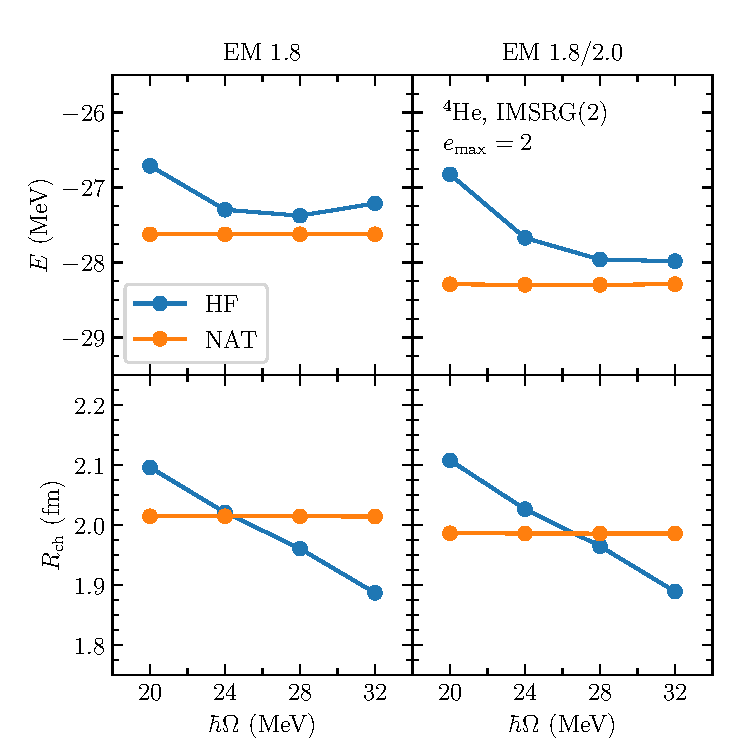
\includegraphics{thesis/doc/images/he4_imsrg2_results}
    \end{center}
    \caption{
        IMSRG(2) ground-state energies (top row) and charge radii (bottom row)
        of ${}^{4}\text{He}$
        for the NN-only EM 1.8 potential (left column)
        and the NN+3N EM 1.8/2.0 potential (right column)
        as a function of the oscillator frequency $\hbar \Omega$
        for the HF and NAT bases.
        The HF basis is constructed in $\emax=2$,
        and the NAT basis is constructed in $\emax=14$,
        with $E_{3\text{max}}=16$ for the NN+3N case,
        before being truncated to $\emax=2$ for the IMSRG(2) calculation.
    }\label{fig:he4_imsrg2_hf_nat}
\end{figure}

In this section,
we take a careful look at what happens to calculations for ${}^{4}\text{He}$
when we apply the IMSRG(3)-$N^7$ truncation.
For reference, we show in Fig.~\ref{fig:he4_imsrg2_hf_nat}
the results for the ground-state energy and charge radius
obtained via the IMSRG(2) for HF and NAT reference states
at various oscillator frequencies.
For the charge radius,
we use the
the square root
of the point-proton mean-square radius operator expectation value
and a spin-orbit correction~\cite{Ong10radius_spin_orbit}
added in quadrature.
We observe that the NAT basis
gives essentially frequency-independent results
for energies and radii
in both the NN-only and NN+3N cases.
The relatively strong frequency dependence
of the HF results is a consequence
of the construction of the HF basis in $\emax=2$.
The correlation energy
\begin{equation}
    E_{\text{corr}}\equiv E(s \rightarrow \infty) - E(s=0)\,,
\end{equation}
which is the contribution to the ground-state energy generated
by the many-body expansion,
is around 4 MeV for the NN-only calculations
and around 5 MeV for the NN+3N calculations.
When we compare the IMSRG(2) and IMSRG(3)-$N^7$ results,
it is sometimes illustrative to consider
their differences relative to $E_{\text{corr}}$,
since $E(s=0)$ is the same in both truncations
and they only differ in their many-body expansion order.
As a concrete example,
for the HF NN+3N case at $\hbar \Omega = 28\mev$,
$E(s=0) = -22.8145\mev$.
For the IMSRG(2) calculation,
$E(s \rightarrow \infty) = -27.9606\mev$
giving a correlation energy of
$E_{\text{corr}} = -5.1461\mev$.

\begin{figure}[t!]
    \begin{center}
        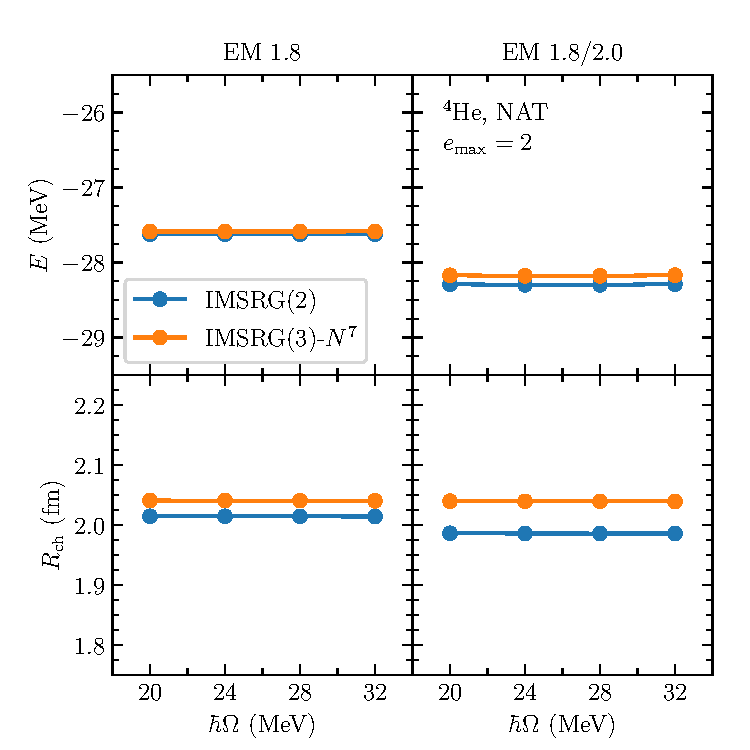
\includegraphics{thesis/doc/images/he4_NAT_results}
    \end{center}
    \caption{
        Ground-state energies (top row) and charge radii (bottom row)
        of ${}^{4}\text{He}$
        for the NN-only EM 1.8 potential (left column)
        and the NN+3N EM 1.8/2.0 potential (right column)
        as a function of the oscillator frequency $\hbar \Omega$
        for the NAT basis
        obtained via IMSRG(2) and IMSRG(3)-$N^7$ calulations.
        The NAT basis is constructed in $\emax=14$,
        with $E_{3\text{max}}=16$ for the NN+3N case,
        before being truncated to $\emax=2$ for the IMSRG calculations.
    }\label{fig:he4_imsrg3_nat}
\end{figure}

\begin{figure}[t!]
    \begin{center}
        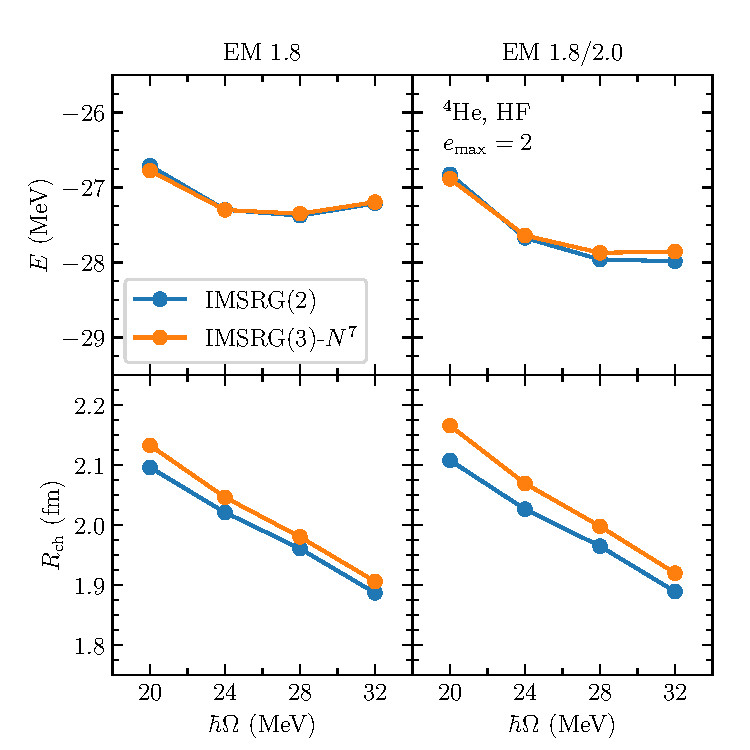
\includegraphics{thesis/doc/images/he4_HF_results}
    \end{center}
    \caption{
        Ground-state energies (top row) and charge radii (bottom row)
        of ${}^{4}\text{He}$
        for the NN-only EM 1.8 potential (left column)
        and the NN+3N EM 1.8/2.0 potential (right column)
        as a function of the oscillator frequency $\hbar \Omega$
        for the HF basis
        obtained via IMSRG(2) and IMSRG(3)-$N^7$ calulations.
        The HF basis is constructed in $\emax=2$.
    }\label{fig:he4_imsrg3_hf}
\end{figure}

The inclusion of 3N forces at the NO2B level gives
(in this system and for this model space)
a slightly larger binding energy
and accordingly a slightly smaller radius.
We emphasize that just the results from $\emax=2$
are not sufficient to make a statement
about the effect of 3N forces in ${}^{4}\text{He}$.
This is because in this model space
the Hamiltonian is not fully converged
with respect to model-space size
and so parts of the Hamiltonian could be cut out by the truncation
that would change the effect of 3N forces.
Thus, to make a concrete claim,
one must also do calculations for larger model spaces (currently out of reach)
and observe that the converged energies
change little as a function of $\emax=2$ to draw conclusions
about the contributions of 3N forces.

Incidentally,
in Jacobi-NCSM calculations, shown in Table~\ref{tab:ncsm_he4_results},
one sees that 3N forces do in fact
give a little bit more binding in ${}^{4}\text{He}$~\cite{Hebe20jac_nscm_he4}.
These values should not be compared with those from our IMSRG calculations
as the extrapolated values are converged with respect to model-space size
while our $\emax=2$ IMSRG results are not,
the $N_{\text{max}}$ truncation used in NCSM calculations
is different from the $\emax$ truncation used in many-body expansion methods,
and the calculation is based additonally on a Jacobi HO basis
instead of a single-particle basis like the single-particle NCSM and the IMSRG.
Additionally,
we use the NO2B approximation here,
which was seen to perform relatively poorly in ${}^{4}\text{He}$
in NCSM calculations~\cite{Roth11nonb_approx}
and is not present in the Jacobi-NCSM calulations discussed above.

In Fig.~\ref{fig:he4_imsrg3_nat},
we compare the results for
the ground-state energy and charge radius of ${}^{4}\text{He}$
for IMSRG(2) and IMSRG(3)-$N^7$ calculations
based on NAT reference states.
The frequency independence of the IMSRG(2) results
is preserved in the IMSRG(3)-$N^7$ results.
The three-body contributions to the ground-state energy
in the IMSRG(3)-$N^7$ are small,
37 keV in the NN-only case
and 120 keV in the NN+3N case.
The effect on the charge radius is more pronounced,
with a shift of 0.026 fm in the NN-only case
and 0.054 fm in the NN+3N case.

In Fig.~\ref{fig:he4_imsrg3_hf},
we see that the same trends are generally seen
for calculations based on HF reference states.
We see that the IMSRG(3)-$N^7$ results
for the energy are slightly flatter
as a function of oscillator frequency
than the IMSRG(2) results.
This may be a sign that the inclusion of three-body operators
in the IMSRG(3)-$N^7$ makes the IMSRG evolution
less sensitive to reference-state deficiencies.
However, to be able to conclude this,
this trend must be seen also for larger model spaces,
for other bases,
and for other closed-shell systems.


\section{Approximate IMSRG(3) truncation-scheme analysis}

\begin{figure}[t!]
    \begin{center}
        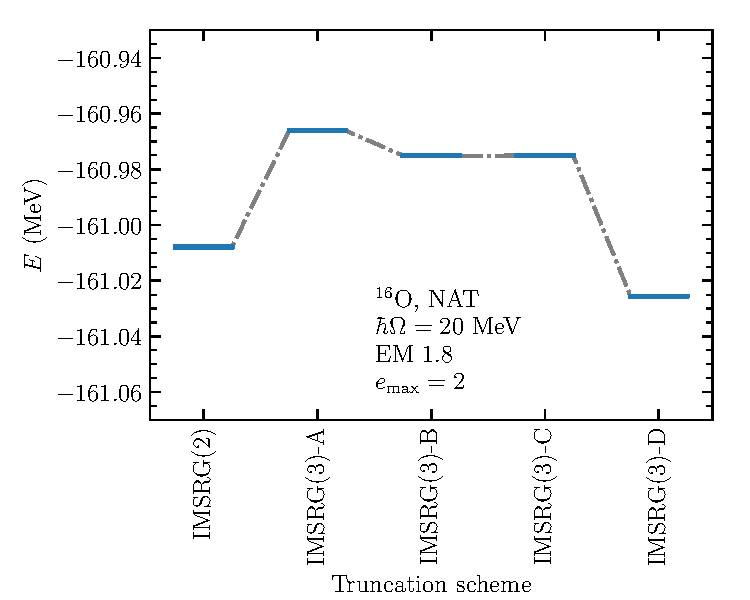
\includegraphics{thesis/doc/images/term_by_term_o16_plot}
    \end{center}
    \caption{
        Ground-state energies
        of ${}^{16}\text{O}$
        for the NN-only EM 1.8 potential
        resulting from IMSRG calculations
        using the IMSRG(2)
        and various approximated IMSRG(3) truncation schemes (see text for details).
        Calculations were done at an oscillator frequency of 20 MeV,
        and a NAT reference state was used.
        The NAT basis is constructed in $\emax=14$
        before being truncated to $\emax=2$ for the various many-body calculations.
    }\label{fig:term_by_term_o16}
\end{figure}

Now we turn our attention to what happens
when we turn on selected fundamental commutators
from the IMSRG(3) relative to the IMSRG(2) starting point.
For the purposes of this first exploration,
we consider ${}^{16}\text{O}$ in an $\emax=2$ model space.
We use the optimized NAT basis,
which delivers essentially frequency-independent results
for IMSRG(2) calculations of ${}^{16}\text{O}$.

In Fig.~\ref{fig:term_by_term_o16},
we show the ground-state energy of
${}^{16}\text{O}$
for various different truncation schemes
(see Sec.~\ref{sec:imsrg3_truncation_schemes} for details).
For all of these calculations, $E_{\text{corr}} \sim 10$ MeV.
We see that the first stable IMSRG(3) approximation,
the IMSRG(3)-A truncation,
produces a sizable shift in the energy of 42 keV.
This is to be contrasted with the next two truncations,
IMSRG(3)-B,
which adds all $\mathcal{O}(N^6)$ IMSRG(3) fundamental commutators
to IMSRG(3)-A,
and IMSRG(3)-C (or IMSRG(3)-$N^7$),
which adds the final remaining $\mathcal{O}(N^7)$ IMSRG(3) fundamental commutator
to IMSRG(3)-B,
where the energy shifts by 9 keV and 0.2 keV respectively.
In this sense,
it seems as though the IMSRG(3)-$N^7$ truncation
is dominated by the commutators included in the IMSRG(3)-A truncation
and the commutators included in the IMSRG(3)-B and IMSRG(3)-C truncations
do relatively little.
We note that for the three commutators added in the IMSRG(3)-B truncation
each commutator separately has a small contribution,
and it is not the case that two commutators have relatively large contributions
that cancel to give an overall small contribution.

The organization outlined in Section~\ref{sec:imsrg3_truncation_schemes}
is primarily based on computational cost.
In light of this organization,
it is interesting that the contribution from the first
$\mathcal{O}(N^8)$ commutator included in the IMSRG(3)-D truncation scheme
is quite large,
producing a 51 keV shift in the ground-state energy.
This suggests that the organization by cost may not be not well motivated
and in practice does not behave desirably when
going from IMSRG(2) to IMSRG(3).
To develop better approximated IMSRG(3) truncation schemes,
one could perform a perturbative analysis as is done in Chapter 7 of Ref.~\cite{Herg15imsrgphysrep}
for IMSRG(2),
where it is shown that IMSRG(2) is exact up to third order in MBPT.
Doing this for IMSRG(3)
would allow one to determine which commutators
to include to make an approximate IMSRG(3) truncation complete
up to some order in MBPT.
